\section{Conclusion}
\label{sec:conclusion}

Procurement authorities need triage tools that work with the data
they already have. The frequent-loser screen delivers: it requires
only win/loss records, runs in minutes on any procurement database,
and flags environments with 3.6--7.7\% higher conditional prices and
strong proximity to known cartels (AUC~$= 0.94$ against
co-participation, surviving exact count matching at $2.2\times$).
Five diagnostics are consistent with coordinated cover bidding.

We propose a three-stage enforcement pathway---addressing the
resource-allocation problem at the heart of antitrust enforcement
since \citet{posner1970statistical}.
(i)~\emph{Screen}---apply the FL rule to participation records.
The computation requires a single table (firm, tender, outcome), no
bid microdata, no enforcement priors, and no supervised training; a
procurement agency can implement it with a SQL query or spreadsheet.
(ii)~\emph{Triage}---cross-reference FL-flagged markets with network
metrics (co-bidding concentration, winner HHI) and oversight-capacity
indicators (PBU size quartile) to prioritize the highest-risk
environments. The 12.5$\times$ gradient in the FL--price association
between the smallest and largest purchasing units suggests that
triage resources are best directed toward low-oversight settings.
(iii)~\emph{Investigate}---deploy bid-level forensic tools
\emph{on the triaged subset}. The screen's near-orthogonality with
bid-level screens (correlation 0.06) means the two stages capture
different collusion signatures, and combining them reduces both
false positives and missed cases.

\begin{figure}[htbp]
\centering
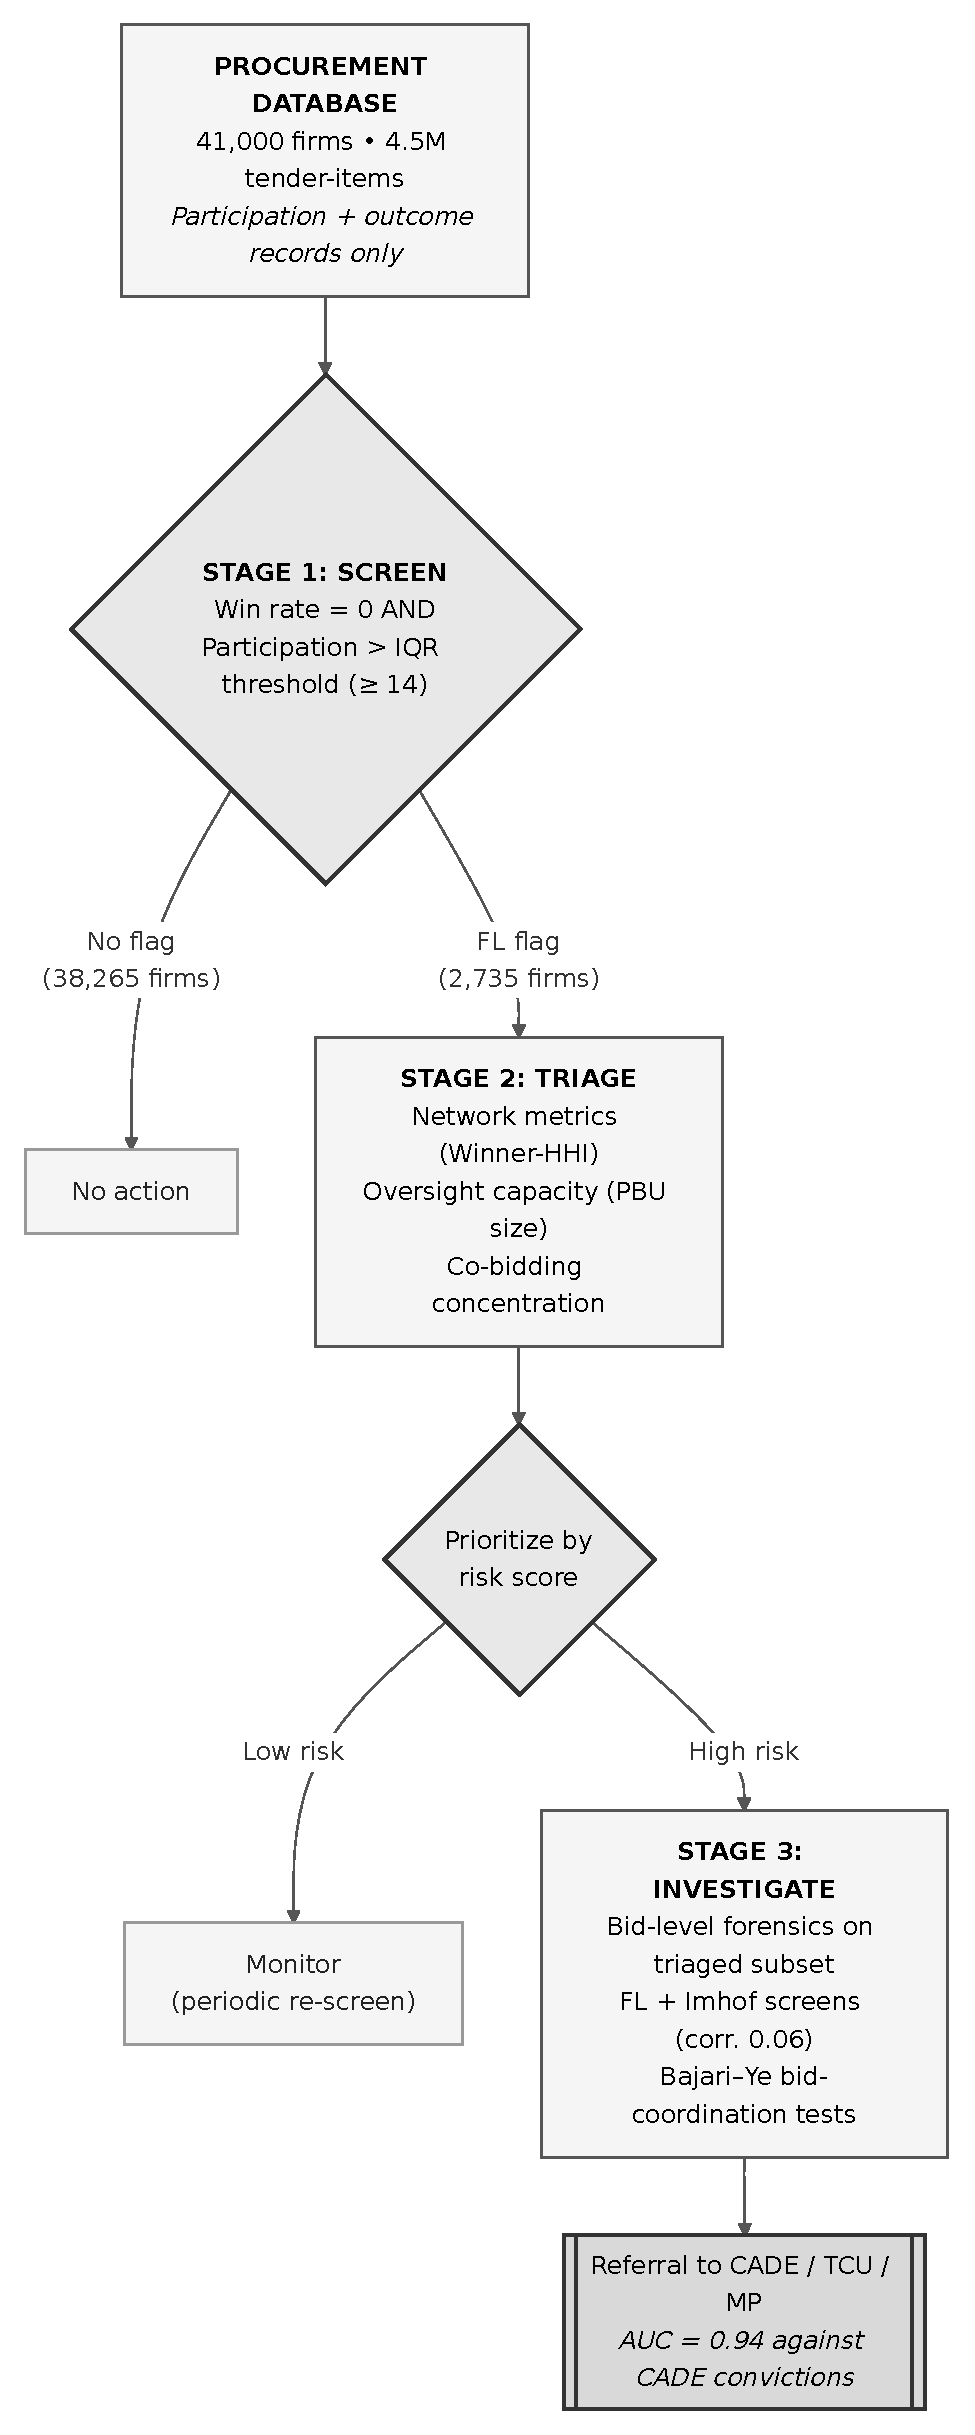
\includegraphics[width=0.45\textwidth]{images/fig_enforcement_flowchart.pdf}
\caption{Three-stage enforcement pathway. Stage~1 reduces 41,000 firms
to 2,735 FL-flagged firms using participation records alone. Stage~2
prioritizes by network structure and oversight capacity. Stage~3
deploys bid-level forensics on the triaged subset.}
\label{fig:enforcement_flowchart}
\end{figure}

Two features make the screen administrable. First, the threshold is
robust: varying the IQR multiplier from 1.0$\times$ to 3.0$\times$
and the win-rate cutoff from 0\% to 5\% yields significant
coefficients across all 36 combinations, so the signal does not
hinge on a precise calibration choice. Second, the data requirements
are minimal---participation and outcome records that every
procurement system already collects---making the screen portable to
developing-country settings where bid-level forensics are out of
reach.

The screen's main limitation is also its defining boundary: it flags
environments, not firms, and the price association is not causal.
These are features of a triage tool, not defects. An enforcement
agency would use it to allocate investigative effort, not to
adjudicate liability. The screen does not replace forensic
investigation; it tells investigators where to start.

The most pressing next step is replication. The economic
logic---cover bidders must participate to perform their role---is
institution-general, but the screen's empirical performance outside
BEC remains to be tested. The FL rule, the ROC analysis, and the
horse-race specification are fully replicable with participation and
outcome data alone.

\paragraph{Institutional change and the new procurement law.}
Brazil's recent procurement reform (Lei~14.133/2021) offers a
natural laboratory. The reform eliminates the convite modality
and with it the minimum-bidder rule that our framework identifies as
a direct incentive for cover bidding. Two predictions follow.
The constraint-binding channel documented in
Section~\ref{sec:additional_id}---where the quorum rule forces
participation and the FL interaction is negative
($\hat{\beta} = -0.160$)---should disappear. The voluntary channel
(7.6\% premium where $n \geq 3$) should survive, since it reflects
strategic choice rather than rule compliance. Comparing pre- and
post-reform procurement within the same item markets would provide a
clean test. The reform also introduces new modalities (di\'alogo
competitivo, concorr\^encia eletr\^onica) with different
participation incentives, and whether the screen works in those
formats is an open question---though it bears noting that the
behavioral footprint the screen exploits (cover bidders must
participate) does not depend on the procurement format.

The reform sharpens the screen's relevance in a broader sense. The
FL--price association is \emph{larger} in preg\~ao (9.3\%) than in
convite (3.8\%), which suggests that cover bidding is not merely a
response to the quorum constraint but a strategic practice that
persists wherever coordination pays. As procurement migrates to
electronic formats under Lei~14.133, participation records will
become richer and more standardized---exactly the data environment
where a participation-based screen has the widest reach. The
transition period, with federal, state, and municipal entities
adopting the new law at different speeds, creates quasi-experimental
variation that future work can use to test portability across
institutional regimes.
